\documentclass[1p]{elsarticle_modified}
%\bibliographystyle{elsarticle-num}

%\usepackage[colorlinks]{hyperref}
%\usepackage{abbrmath_seonhwa} %\Abb, \Ascr, \Acal ,\Abf, \Afrak
\usepackage{amsfonts}
\usepackage{amssymb}
\usepackage{amsmath}
\usepackage{amsthm}
\usepackage{scalefnt}
\usepackage{amsbsy}
\usepackage{kotex}
\usepackage{caption}
\usepackage{subfig}
\usepackage{color}
\usepackage{graphicx}
\usepackage{xcolor} %% white, black, red, green, blue, cyan, magenta, yellow
\usepackage{float}
\usepackage{setspace}
\usepackage{hyperref}

\usepackage{tikz}
\usetikzlibrary{arrows}

\usepackage{multirow}
\usepackage{array} % fixed length table
\usepackage{hhline}

%%%%%%%%%%%%%%%%%%%%%
\makeatletter
\renewcommand*\env@matrix[1][\arraystretch]{%
	\edef\arraystretch{#1}%
	\hskip -\arraycolsep
	\let\@ifnextchar\new@ifnextchar
	\array{*\c@MaxMatrixCols c}}
\makeatother %https://tex.stackexchange.com/questions/14071/how-can-i-increase-the-line-spacing-in-a-matrix
%%%%%%%%%%%%%%%

\usepackage[normalem]{ulem}

\newcommand{\msout}[1]{\ifmmode\text{\sout{\ensuremath{#1}}}\else\sout{#1}\fi}
%SOURCE: \msout is \stkout macro in https://tex.stackexchange.com/questions/20609/strikeout-in-math-mode

\newcommand{\cancel}[1]{
	\ifmmode
	{\color{red}\msout{#1}}
	\else
	{\color{red}\sout{#1}}
	\fi
}

\newcommand{\add}[1]{
	{\color{blue}\uwave{#1}}
}

\newcommand{\replace}[2]{
	\ifmmode
	{\color{red}\msout{#1}}{\color{blue}\uwave{#2}}
	\else
	{\color{red}\sout{#1}}{\color{blue}\uwave{#2}}
	\fi
}

\newcommand{\Sol}{\mathcal{S}} %segment
\newcommand{\D}{D} %diagram
\newcommand{\A}{\mathcal{A}} %arc


%%%%%%%%%%%%%%%%%%%%%%%%%%%%%5 test

\def\sl{\operatorname{\textup{SL}}(2,\Cbb)}
\def\psl{\operatorname{\textup{PSL}}(2,\Cbb)}
\def\quan{\mkern 1mu \triangleright \mkern 1mu}

\theoremstyle{definition}
\newtheorem{thm}{Theorem}[section]
\newtheorem{prop}[thm]{Proposition}
\newtheorem{lem}[thm]{Lemma}
\newtheorem{ques}[thm]{Question}
\newtheorem{cor}[thm]{Corollary}
\newtheorem{defn}[thm]{Definition}
\newtheorem{exam}[thm]{Example}
\newtheorem{rmk}[thm]{Remark}
\newtheorem{alg}[thm]{Algorithm}

\newcommand{\I}{\sqrt{-1}}
\begin{document}

%\begin{frontmatter}
%
%\title{Boundary parabolic representations of knots up to 8 crossings}
%
%%% Group authors per affiliation:
%\author{Yunhi Cho} 
%\address{Department of Mathematics, University of Seoul, Seoul, Korea}
%\ead{yhcho@uos.ac.kr}
%
%
%\author{Seonhwa Kim} %\fnref{s_kim}}
%\address{Center for Geometry and Physics, Institute for Basic Science, Pohang, 37673, Korea}
%\ead{ryeona17@ibs.re.kr}
%
%\author{Hyuk Kim}
%\address{Department of Mathematical Sciences, Seoul National University, Seoul 08826, Korea}
%\ead{hyukkim@snu.ac.kr}
%
%\author{Seokbeom Yoon}
%\address{Department of Mathematical Sciences, Seoul National University, Seoul, 08826,  Korea}
%\ead{sbyoon15@snu.ac.kr}
%
%\begin{abstract}
%We find all boundary parabolic representation of knots up to 8 crossings.
%
%\end{abstract}
%\begin{keyword}
%    \MSC[2010] 57M25 
%\end{keyword}
%
%\end{frontmatter}

%\linenumbers
%\tableofcontents
%
\newcommand\colored[1]{\textcolor{white}{\rule[-0.35ex]{0.8em}{1.4ex}}\kern-0.8em\color{red} #1}%
%\newcommand\colored[1]{\textcolor{white}{ #1}\kern-2.17ex	\textcolor{white}{ #1}\kern-1.81ex	\textcolor{white}{ #1}\kern-2.15ex\color{red}#1	}

{\Large $\underline{12a_{0947}~(K12a_{0947})}$}

\setlength{\tabcolsep}{10pt}
\renewcommand{\arraystretch}{1.6}
\vspace{1cm}\begin{tabular}{m{100pt}>{\centering\arraybackslash}m{274pt}}
\multirow{5}{120pt}{
	\centering
	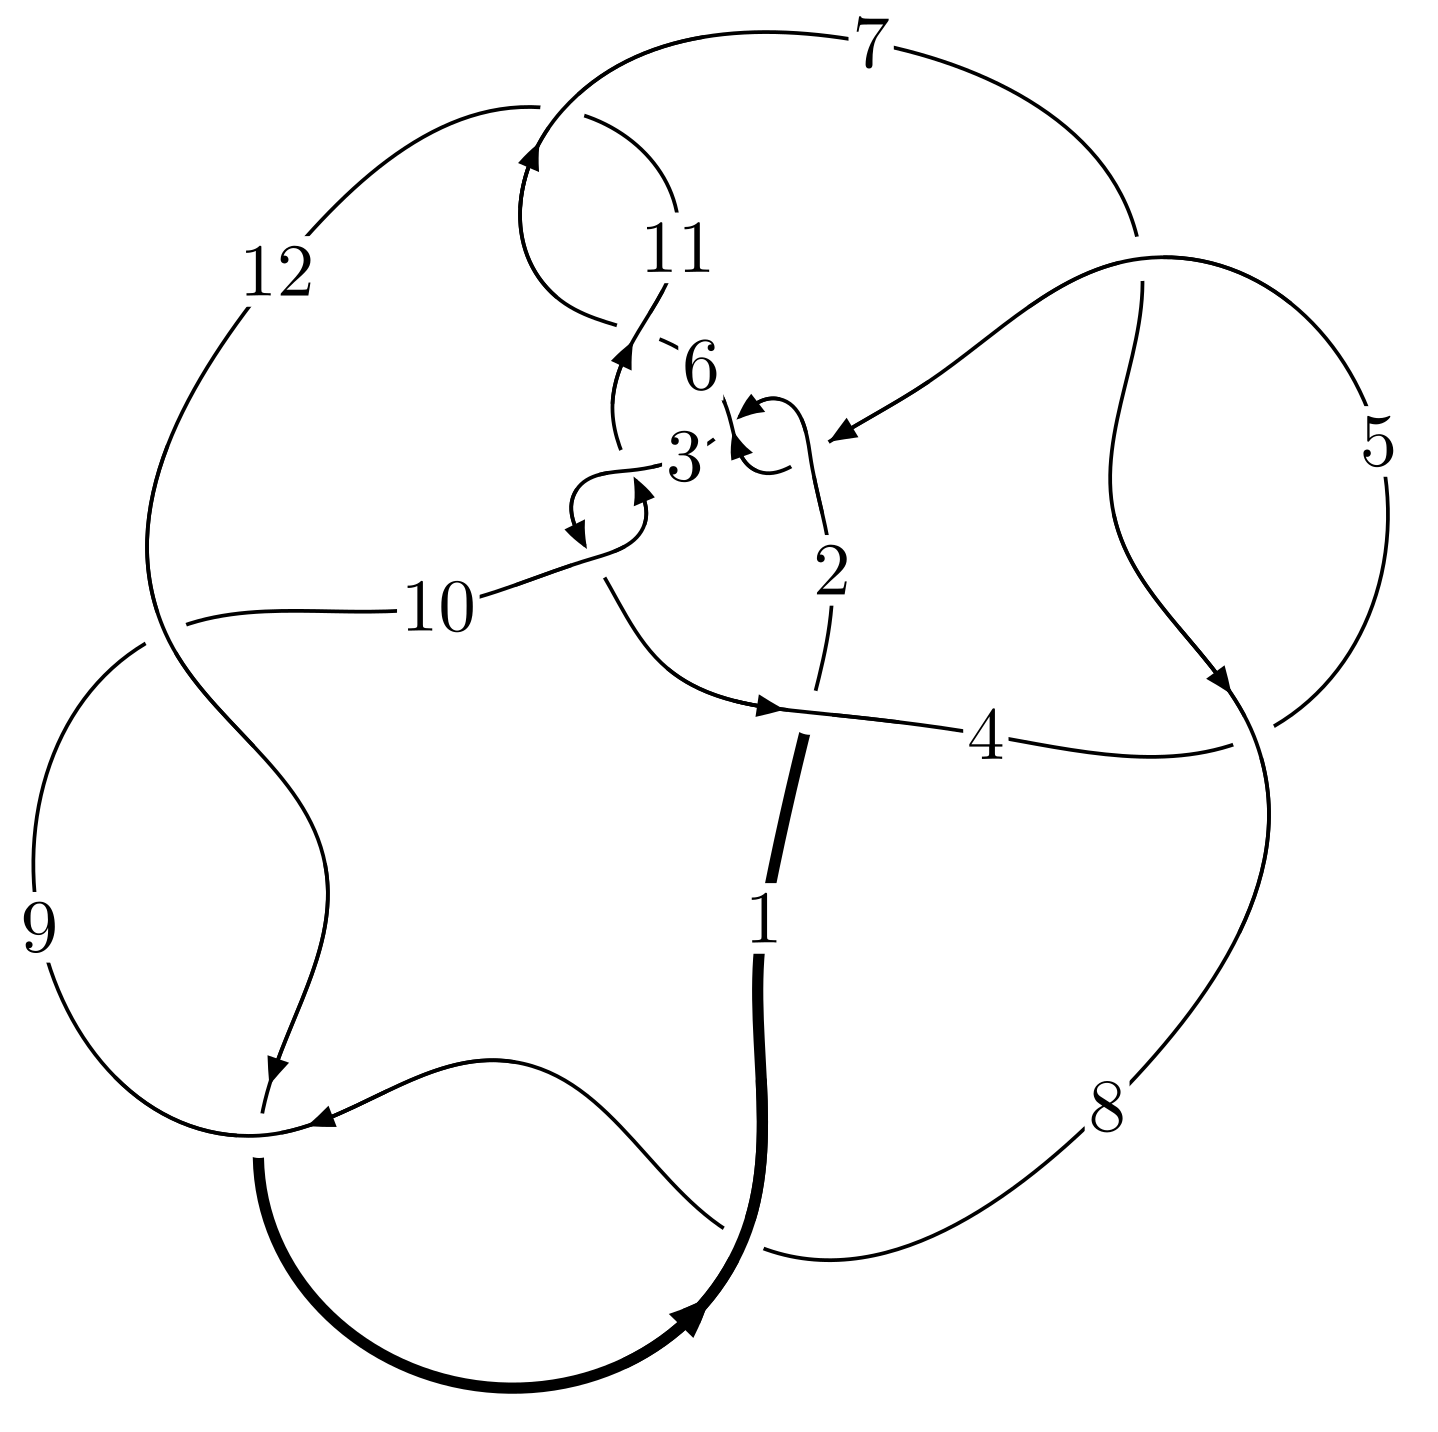
\includegraphics[width=112pt]{../../../GIT/diagram.site/Diagrams/png/1748_12a_0947.png}\\
\ \ \ A knot diagram\footnotemark}&
\allowdisplaybreaks
\textbf{Linearized knot diagam} \\
\cline{2-2}
 &
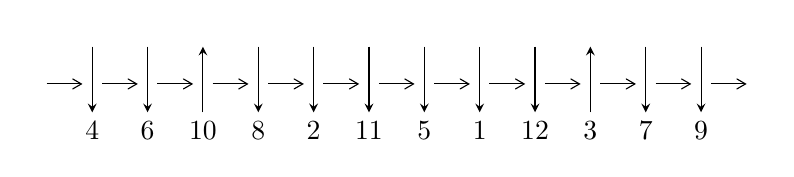
\begin{tikzpicture}[x=20pt, y=17pt]
	% nodes
	\node (C0) at (0, 0) {};
	\node (C1) at (1, 0) {};
	\node (C1U) at (1, +1) {};
	\node (C1D) at (1, -1) {4};

	\node (C2) at (2, 0) {};
	\node (C2U) at (2, +1) {};
	\node (C2D) at (2, -1) {6};

	\node (C3) at (3, 0) {};
	\node (C3U) at (3, +1) {};
	\node (C3D) at (3, -1) {10};

	\node (C4) at (4, 0) {};
	\node (C4U) at (4, +1) {};
	\node (C4D) at (4, -1) {8};

	\node (C5) at (5, 0) {};
	\node (C5U) at (5, +1) {};
	\node (C5D) at (5, -1) {2};

	\node (C6) at (6, 0) {};
	\node (C6U) at (6, +1) {};
	\node (C6D) at (6, -1) {11};

	\node (C7) at (7, 0) {};
	\node (C7U) at (7, +1) {};
	\node (C7D) at (7, -1) {5};

	\node (C8) at (8, 0) {};
	\node (C8U) at (8, +1) {};
	\node (C8D) at (8, -1) {1};

	\node (C9) at (9, 0) {};
	\node (C9U) at (9, +1) {};
	\node (C9D) at (9, -1) {12};

	\node (C10) at (10, 0) {};
	\node (C10U) at (10, +1) {};
	\node (C10D) at (10, -1) {3};

	\node (C11) at (11, 0) {};
	\node (C11U) at (11, +1) {};
	\node (C11D) at (11, -1) {7};

	\node (C12) at (12, 0) {};
	\node (C12U) at (12, +1) {};
	\node (C12D) at (12, -1) {9};
	\node (C13) at (13, 0) {};

	% arrows
	\draw[->,>={angle 60}]
	(C0) edge (C1) (C1) edge (C2) (C2) edge (C3) (C3) edge (C4) (C4) edge (C5) (C5) edge (C6) (C6) edge (C7) (C7) edge (C8) (C8) edge (C9) (C9) edge (C10) (C10) edge (C11) (C11) edge (C12) (C12) edge (C13) ;	\draw[->,>=stealth]
	(C1U) edge (C1D) (C2U) edge (C2D) (C3D) edge (C3U) (C4U) edge (C4D) (C5U) edge (C5D) (C6U) edge (C6D) (C7U) edge (C7D) (C8U) edge (C8D) (C9U) edge (C9D) (C10D) edge (C10U) (C11U) edge (C11D) (C12U) edge (C12D) ;
	\end{tikzpicture} \\
\hhline{~~} \\& 
\textbf{Solving Sequence} \\ \cline{2-2} 
 &
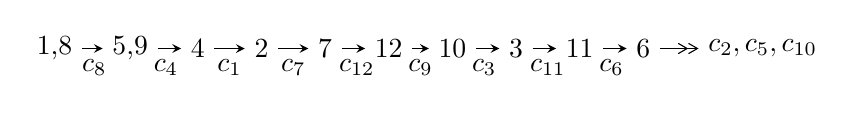
\begin{tikzpicture}[x=23pt, y=7pt]
	% node
	\node (A0) at (-1/8, 0) {1,8};
	\node (A1) at (17/16, 0) {5,9};
	\node (A2) at (17/8, 0) {4};
	\node (A3) at (25/8, 0) {2};
	\node (A4) at (33/8, 0) {7};
	\node (A5) at (41/8, 0) {12};
	\node (A6) at (49/8, 0) {10};
	\node (A7) at (57/8, 0) {3};
	\node (A8) at (65/8, 0) {11};
	\node (A9) at (73/8, 0) {6};
	\node (C1) at (1/2, -1) {$c_{8}$};
	\node (C2) at (13/8, -1) {$c_{4}$};
	\node (C3) at (21/8, -1) {$c_{1}$};
	\node (C4) at (29/8, -1) {$c_{7}$};
	\node (C5) at (37/8, -1) {$c_{12}$};
	\node (C6) at (45/8, -1) {$c_{9}$};
	\node (C7) at (53/8, -1) {$c_{3}$};
	\node (C8) at (61/8, -1) {$c_{11}$};
	\node (C9) at (69/8, -1) {$c_{6}$};
	\node (A10) at (11, 0) {$c_{2},c_{5},c_{10}$};

	% edge
	\draw[->,>=stealth]	
	(A0) edge (A1) (A1) edge (A2) (A2) edge (A3) (A3) edge (A4) (A4) edge (A5) (A5) edge (A6) (A6) edge (A7) (A7) edge (A8) (A8) edge (A9) ;
	\draw[->>,>={angle 60}]	
	(A9) edge (A10);
\end{tikzpicture} \\ 

\end{tabular} \\

\footnotetext{
The image of knot diagram is generated by the software ``\textbf{Draw programme}" developed by Andrew Bartholomew(\url{http://www.layer8.co.uk/maths/draw/index.htm\#Running-draw}), where we modified some parts for our purpose(\url{https://github.com/CATsTAILs/LinksPainter}).
}\phantom \\ \newline 
\centering \textbf{Ideals for irreducible components\footnotemark of $X_{\text{par}}$} 
 
\begin{align*}
I^u_{1}&=\langle 
7.66580\times10^{216} u^{95}+3.01207\times10^{217} u^{94}+\cdots+1.39904\times10^{215} b-6.84600\times10^{217},\\
\phantom{I^u_{1}}&\phantom{= \langle  }1.29437\times10^{218} u^{95}+5.06589\times10^{218} u^{94}+\cdots+1.39904\times10^{215} a-1.09950\times10^{219},\;u^{96}+4 u^{95}+\cdots-25 u-1\rangle \\
I^u_{2}&=\langle 
1711 u^{17}-5392 u^{16}+\cdots+2500 b-6081,\;-3773 u^{17}+11256 u^{16}+\cdots+2500 a+13183,\\
\phantom{I^u_{2}}&\phantom{= \langle  }u^{18}-3 u^{17}+\cdots-8 u+1\rangle \\
\\
\end{align*}
\raggedright * 2 irreducible components of $\dim_{\mathbb{C}}=0$, with total 114 representations.\\
\footnotetext{All coefficients of polynomials are rational numbers. But the coefficients are sometimes approximated in decimal forms when there is not enough margin.}
\newpage
\renewcommand{\arraystretch}{1}
\centering \section*{I. $I^u_{1}= \langle 7.67\times10^{216} u^{95}+3.01\times10^{217} u^{94}+\cdots+1.40\times10^{215} b-6.85\times10^{217},\;1.29\times10^{218} u^{95}+5.07\times10^{218} u^{94}+\cdots+1.40\times10^{215} a-1.10\times10^{219},\;u^{96}+4 u^{95}+\cdots-25 u-1 \rangle$}
\flushleft \textbf{(i) Arc colorings}\\
\begin{tabular}{m{7pt} m{180pt} m{7pt} m{180pt} }
\flushright $a_{1}=$&$\begin{pmatrix}0\\u\end{pmatrix}$ \\
\flushright $a_{8}=$&$\begin{pmatrix}1\\0\end{pmatrix}$ \\
\flushright $a_{5}=$&$\begin{pmatrix}-925.186 u^{95}-3620.99 u^{94}+\cdots+138205. u+7859.01\\-54.7935 u^{95}-215.296 u^{94}+\cdots+8402.17 u+489.337\end{pmatrix}$ \\
\flushright $a_{9}=$&$\begin{pmatrix}1\\u^2\end{pmatrix}$ \\
\flushright $a_{4}=$&$\begin{pmatrix}-979.980 u^{95}-3836.28 u^{94}+\cdots+146607. u+8348.35\\-54.7935 u^{95}-215.296 u^{94}+\cdots+8402.17 u+489.337\end{pmatrix}$ \\
\flushright $a_{2}=$&$\begin{pmatrix}3187.09 u^{95}+12055.6 u^{94}+\cdots-285324. u-13138.4\\-336.870 u^{95}-1289.44 u^{94}+\cdots+36955.3 u+1887.42\end{pmatrix}$ \\
\flushright $a_{7}=$&$\begin{pmatrix}1579.76 u^{95}+6036.96 u^{94}+\cdots-169129. u-8544.27\\307.658 u^{95}+1175.84 u^{94}+\cdots-33247.8 u-1685.90\end{pmatrix}$ \\
\flushright $a_{12}=$&$\begin{pmatrix}u\\u^3+u\end{pmatrix}$ \\
\flushright $a_{10}=$&$\begin{pmatrix}u^2+1\\u^4+2 u^2\end{pmatrix}$ \\
\flushright $a_{3}=$&$\begin{pmatrix}-920.556 u^{95}-3608.52 u^{94}+\cdots+140115. u+8009.42\\-51.2527 u^{95}-201.384 u^{94}+\cdots+8012.54 u+469.142\end{pmatrix}$ \\
\flushright $a_{11}=$&$\begin{pmatrix}3385.53 u^{95}+12905.7 u^{94}+\cdots-348333. u-17274.1\\200.126 u^{95}+764.543 u^{94}+\cdots-21202.5 u-1065.35\end{pmatrix}$ \\
\flushright $a_{6}=$&$\begin{pmatrix}-3201.35 u^{95}-12106.0 u^{94}+\cdots+285009. u+13082.2\\348.559 u^{95}+1334.10 u^{94}+\cdots-38296.5 u-1957.71\end{pmatrix}$\\&\end{tabular}
\flushleft \textbf{(ii) Obstruction class $= -1$}\\~\\
\flushleft \textbf{(iii) Cusp Shapes $= -1561.38 u^{95}-5923.49 u^{94}+\cdots+147695. u+7028.63$}\\~\\
\newpage\renewcommand{\arraystretch}{1}
\flushleft \textbf{(iv) u-Polynomials at the component}\newline \\
\begin{tabular}{m{50pt}|m{274pt}}
Crossings & \hspace{64pt}u-Polynomials at each crossing \\
\hline $$\begin{aligned}c_{1}\end{aligned}$$&$\begin{aligned}
&u^{96}-12 u^{95}+\cdots+50079 u-22271
\end{aligned}$\\
\hline $$\begin{aligned}c_{2},c_{5}\end{aligned}$$&$\begin{aligned}
&u^{96}+u^{95}+\cdots+22242 u-604
\end{aligned}$\\
\hline $$\begin{aligned}c_{3},c_{10}\end{aligned}$$&$\begin{aligned}
&u^{96}+u^{95}+\cdots-12111 u+11963
\end{aligned}$\\
\hline $$\begin{aligned}c_{4},c_{7}\end{aligned}$$&$\begin{aligned}
&u^{96}-8 u^{95}+\cdots+2325 u+599
\end{aligned}$\\
\hline $$\begin{aligned}c_{6},c_{11}\end{aligned}$$&$\begin{aligned}
&u^{96}- u^{95}+\cdots+29368 u+2361
\end{aligned}$\\
\hline $$\begin{aligned}c_{8},c_{9},c_{12}\end{aligned}$$&$\begin{aligned}
&u^{96}-4 u^{95}+\cdots+25 u-1
\end{aligned}$\\
\hline
\end{tabular}\\~\\
\newpage\renewcommand{\arraystretch}{1}
\flushleft \textbf{(v) Riley Polynomials at the component}\newline \\
\begin{tabular}{m{50pt}|m{274pt}}
Crossings & \hspace{64pt}Riley Polynomials at each crossing \\
\hline $$\begin{aligned}c_{1}\end{aligned}$$&$\begin{aligned}
&y^{96}+22 y^{95}+\cdots+13135555953 y+495997441
\end{aligned}$\\
\hline $$\begin{aligned}c_{2},c_{5}\end{aligned}$$&$\begin{aligned}
&y^{96}-79 y^{95}+\cdots-781387916 y+364816
\end{aligned}$\\
\hline $$\begin{aligned}c_{3},c_{10}\end{aligned}$$&$\begin{aligned}
&y^{96}+83 y^{95}+\cdots-3976989661 y+143113369
\end{aligned}$\\
\hline $$\begin{aligned}c_{4},c_{7}\end{aligned}$$&$\begin{aligned}
&y^{96}+74 y^{95}+\cdots+27105699 y+358801
\end{aligned}$\\
\hline $$\begin{aligned}c_{6},c_{11}\end{aligned}$$&$\begin{aligned}
&y^{96}-73 y^{95}+\cdots-1783425250 y+5574321
\end{aligned}$\\
\hline $$\begin{aligned}c_{8},c_{9},c_{12}\end{aligned}$$&$\begin{aligned}
&y^{96}+98 y^{95}+\cdots-125 y+1
\end{aligned}$\\
\hline
\end{tabular}\\~\\
\newpage\flushleft \textbf{(vi) Complex Volumes and Cusp Shapes}
$$\begin{array}{c|c|c}  
\text{Solutions to }I^u_{1}& \I (\text{vol} + \sqrt{-1}CS) & \text{Cusp shape}\\
 \hline 
\begin{aligned}
u &= \phantom{-}0.668054 + 0.736176 I \\
a &= -0.429663 + 0.886280 I \\
b &= -0.273010 - 1.079940 I\end{aligned}
 & \phantom{-}1.87671 - 3.14768 I & \phantom{-0.000000 } 0 \\ \hline\begin{aligned}
u &= \phantom{-}0.668054 - 0.736176 I \\
a &= -0.429663 - 0.886280 I \\
b &= -0.273010 + 1.079940 I\end{aligned}
 & \phantom{-}1.87671 + 3.14768 I & \phantom{-0.000000 } 0 \\ \hline\begin{aligned}
u &= \phantom{-}0.774207 + 0.606189 I \\
a &= \phantom{-}0.915311 - 0.669410 I \\
b &= \phantom{-}0.133604 + 1.038010 I\end{aligned}
 & \phantom{-}1.49646 - 2.68540 I & \phantom{-0.000000 } 0 \\ \hline\begin{aligned}
u &= \phantom{-}0.774207 - 0.606189 I \\
a &= \phantom{-}0.915311 + 0.669410 I \\
b &= \phantom{-}0.133604 - 1.038010 I\end{aligned}
 & \phantom{-}1.49646 + 2.68540 I & \phantom{-0.000000 } 0 \\ \hline\begin{aligned}
u &= -0.498397 + 0.839577 I \\
a &= -0.08073 + 1.53160 I \\
b &= \phantom{-}0.574093 - 0.358999 I\end{aligned}
 & -8.84762 - 2.96103 I & \phantom{-0.000000 } 0 \\ \hline\begin{aligned}
u &= -0.498397 - 0.839577 I \\
a &= -0.08073 - 1.53160 I \\
b &= \phantom{-}0.574093 + 0.358999 I\end{aligned}
 & -8.84762 + 2.96103 I & \phantom{-0.000000 } 0 \\ \hline\begin{aligned}
u &= -0.906591 + 0.538873 I \\
a &= \phantom{-}0.708668 + 0.801467 I \\
b &= \phantom{-}0.539203 - 1.263990 I\end{aligned}
 & -6.8746 + 12.7575 I & \phantom{-0.000000 } 0 \\ \hline\begin{aligned}
u &= -0.906591 - 0.538873 I \\
a &= \phantom{-}0.708668 - 0.801467 I \\
b &= \phantom{-}0.539203 + 1.263990 I\end{aligned}
 & -6.8746 - 12.7575 I & \phantom{-0.000000 } 0 \\ \hline\begin{aligned}
u &= \phantom{-}0.642962 + 0.634792 I \\
a &= \phantom{-}0.705564 - 0.816030 I \\
b &= \phantom{-}0.614653 + 1.195540 I\end{aligned}
 & -1.62318 - 7.04624 I & \phantom{-0.000000 } 0 \\ \hline\begin{aligned}
u &= \phantom{-}0.642962 - 0.634792 I \\
a &= \phantom{-}0.705564 + 0.816030 I \\
b &= \phantom{-}0.614653 - 1.195540 I\end{aligned}
 & -1.62318 + 7.04624 I & \phantom{-0.000000 } 0\\
 \hline 
 \end{array}$$\newpage$$\begin{array}{c|c|c}  
\text{Solutions to }I^u_{1}& \I (\text{vol} + \sqrt{-1}CS) & \text{Cusp shape}\\
 \hline 
\begin{aligned}
u &= \phantom{-}0.823842 + 0.327264 I \\
a &= -0.400902 - 0.137615 I \\
b &= \phantom{-}0.345374 - 0.991459 I\end{aligned}
 & -2.63541 + 2.26716 I & \phantom{-0.000000 } 0 \\ \hline\begin{aligned}
u &= \phantom{-}0.823842 - 0.327264 I \\
a &= -0.400902 + 0.137615 I \\
b &= \phantom{-}0.345374 + 0.991459 I\end{aligned}
 & -2.63541 - 2.26716 I & \phantom{-0.000000 } 0 \\ \hline\begin{aligned}
u &= \phantom{-}0.667116 + 0.468592 I \\
a &= -1.53049 + 0.79417 I \\
b &= -0.411037 - 1.217960 I\end{aligned}
 & -1.76974 - 6.29232 I & \phantom{-0.000000 } 0 \\ \hline\begin{aligned}
u &= \phantom{-}0.667116 - 0.468592 I \\
a &= -1.53049 - 0.79417 I \\
b &= -0.411037 + 1.217960 I\end{aligned}
 & -1.76974 + 6.29232 I & \phantom{-0.000000 } 0 \\ \hline\begin{aligned}
u &= -0.979656 + 0.724547 I \\
a &= -0.444493 - 0.520408 I \\
b &= \phantom{-}0.354693 + 1.111030 I\end{aligned}
 & -6.48587 - 6.61272 I & \phantom{-0.000000 } 0 \\ \hline\begin{aligned}
u &= -0.979656 - 0.724547 I \\
a &= -0.444493 + 0.520408 I \\
b &= \phantom{-}0.354693 - 1.111030 I\end{aligned}
 & -6.48587 + 6.61272 I & \phantom{-0.000000 } 0 \\ \hline\begin{aligned}
u &= \phantom{-}0.273545 + 1.199010 I \\
a &= -0.019882 + 0.518557 I \\
b &= -0.154446 - 0.611071 I\end{aligned}
 & \phantom{-}2.09188 - 2.59239 I & \phantom{-0.000000 } 0 \\ \hline\begin{aligned}
u &= \phantom{-}0.273545 - 1.199010 I \\
a &= -0.019882 - 0.518557 I \\
b &= -0.154446 + 0.611071 I\end{aligned}
 & \phantom{-}2.09188 + 2.59239 I & \phantom{-0.000000 } 0 \\ \hline\begin{aligned}
u &= -0.696468 + 0.319796 I \\
a &= \phantom{-}0.387796 - 0.165500 I \\
b &= \phantom{-}1.049040 + 0.160137 I\end{aligned}
 & -10.34670 + 7.16521 I & \phantom{-0.000000 } 0 \\ \hline\begin{aligned}
u &= -0.696468 - 0.319796 I \\
a &= \phantom{-}0.387796 + 0.165500 I \\
b &= \phantom{-}1.049040 - 0.160137 I\end{aligned}
 & -10.34670 - 7.16521 I & \phantom{-0.000000 } 0\\
 \hline 
 \end{array}$$\newpage$$\begin{array}{c|c|c}  
\text{Solutions to }I^u_{1}& \I (\text{vol} + \sqrt{-1}CS) & \text{Cusp shape}\\
 \hline 
\begin{aligned}
u &= -1.163950 + 0.429343 I \\
a &= -0.338442 - 0.653919 I \\
b &= -0.239374 + 1.220300 I\end{aligned}
 & -0.75881 + 5.38751 I & \phantom{-0.000000 } 0 \\ \hline\begin{aligned}
u &= -1.163950 - 0.429343 I \\
a &= -0.338442 + 0.653919 I \\
b &= -0.239374 - 1.220300 I\end{aligned}
 & -0.75881 - 5.38751 I & \phantom{-0.000000 } 0 \\ \hline\begin{aligned}
u &= \phantom{-}0.590524 + 0.473244 I \\
a &= -0.555181 + 0.658882 I \\
b &= -0.786117 - 0.003987 I\end{aligned}
 & -5.43999 - 2.01203 I & \phantom{-0.000000 } 0 \\ \hline\begin{aligned}
u &= \phantom{-}0.590524 - 0.473244 I \\
a &= -0.555181 - 0.658882 I \\
b &= -0.786117 + 0.003987 I\end{aligned}
 & -5.43999 + 2.01203 I & \phantom{-0.000000 } 0 \\ \hline\begin{aligned}
u &= -0.334446 + 1.211940 I \\
a &= \phantom{-}0.436652 - 0.624605 I \\
b &= -0.0686828 - 0.1203880 I\end{aligned}
 & -1.64270 + 1.53619 I & \phantom{-0.000000 } 0 \\ \hline\begin{aligned}
u &= -0.334446 - 1.211940 I \\
a &= \phantom{-}0.436652 + 0.624605 I \\
b &= -0.0686828 + 0.1203880 I\end{aligned}
 & -1.64270 - 1.53619 I & \phantom{-0.000000 } 0 \\ \hline\begin{aligned}
u &= -0.239165 + 1.236350 I \\
a &= -0.960999 + 0.305868 I \\
b &= \phantom{-}0.062907 + 0.929306 I\end{aligned}
 & -3.21662 + 4.59968 I & \phantom{-0.000000 } 0 \\ \hline\begin{aligned}
u &= -0.239165 - 1.236350 I \\
a &= -0.960999 - 0.305868 I \\
b &= \phantom{-}0.062907 - 0.929306 I\end{aligned}
 & -3.21662 - 4.59968 I & \phantom{-0.000000 } 0 \\ \hline\begin{aligned}
u &= -0.718935 + 0.159858 I \\
a &= -0.424784 + 0.609798 I \\
b &= -0.625472 + 0.146870 I\end{aligned}
 & -4.80317 + 2.40591 I & \phantom{-0.000000 } 0 \\ \hline\begin{aligned}
u &= -0.718935 - 0.159858 I \\
a &= -0.424784 - 0.609798 I \\
b &= -0.625472 - 0.146870 I\end{aligned}
 & -4.80317 - 2.40591 I & \phantom{-0.000000 } 0\\
 \hline 
 \end{array}$$\newpage$$\begin{array}{c|c|c}  
\text{Solutions to }I^u_{1}& \I (\text{vol} + \sqrt{-1}CS) & \text{Cusp shape}\\
 \hline 
\begin{aligned}
u &= \phantom{-}0.598357 + 0.380180 I \\
a &= \phantom{-}0.210313 - 0.387022 I \\
b &= -0.363056 + 1.191810 I\end{aligned}
 & -1.82836 + 2.13302 I & \phantom{-0.000000 } 0 \\ \hline\begin{aligned}
u &= \phantom{-}0.598357 - 0.380180 I \\
a &= \phantom{-}0.210313 + 0.387022 I \\
b &= -0.363056 - 1.191810 I\end{aligned}
 & -1.82836 - 2.13302 I & \phantom{-0.000000 } 0 \\ \hline\begin{aligned}
u &= -0.388642 + 0.581905 I \\
a &= \phantom{-}1.232050 + 0.617206 I \\
b &= \phantom{-}0.004208 - 1.122470 I\end{aligned}
 & \phantom{-}3.09946 - 0.88819 I & \phantom{-0.000000 } 0 \\ \hline\begin{aligned}
u &= -0.388642 - 0.581905 I \\
a &= \phantom{-}1.232050 - 0.617206 I \\
b &= \phantom{-}0.004208 + 1.122470 I\end{aligned}
 & \phantom{-}3.09946 + 0.88819 I & \phantom{-0.000000 } 0 \\ \hline\begin{aligned}
u &= -0.200518 + 1.292240 I \\
a &= \phantom{-}0.808068 + 0.422740 I \\
b &= \phantom{-}0.629734 - 0.807012 I\end{aligned}
 & -2.97629 + 1.71649 I & \phantom{-0.000000 } 0 \\ \hline\begin{aligned}
u &= -0.200518 - 1.292240 I \\
a &= \phantom{-}0.808068 - 0.422740 I \\
b &= \phantom{-}0.629734 + 0.807012 I\end{aligned}
 & -2.97629 - 1.71649 I & \phantom{-0.000000 } 0 \\ \hline\begin{aligned}
u &= -0.651902 + 0.011051 I \\
a &= \phantom{-}0.48383 - 1.60027 I \\
b &= \phantom{-}0.358350 - 0.916006 I\end{aligned}
 & -6.96647 - 1.33186 I & \phantom{-0.000000 } 0 \\ \hline\begin{aligned}
u &= -0.651902 - 0.011051 I \\
a &= \phantom{-}0.48383 + 1.60027 I \\
b &= \phantom{-}0.358350 + 0.916006 I\end{aligned}
 & -6.96647 + 1.33186 I & \phantom{-0.000000 } 0 \\ \hline\begin{aligned}
u &= -0.067232 + 1.355170 I \\
a &= \phantom{-}0.658539 - 0.383013 I \\
b &= \phantom{-}0.681245 + 0.819076 I\end{aligned}
 & -2.94394 - 3.38274 I & \phantom{-0.000000 } 0 \\ \hline\begin{aligned}
u &= -0.067232 - 1.355170 I \\
a &= \phantom{-}0.658539 + 0.383013 I \\
b &= \phantom{-}0.681245 - 0.819076 I\end{aligned}
 & -2.94394 + 3.38274 I & \phantom{-0.000000 } 0\\
 \hline 
 \end{array}$$\newpage$$\begin{array}{c|c|c}  
\text{Solutions to }I^u_{1}& \I (\text{vol} + \sqrt{-1}CS) & \text{Cusp shape}\\
 \hline 
\begin{aligned}
u &= -0.012508 + 1.365180 I \\
a &= \phantom{-}0.467529 + 1.277170 I \\
b &= -1.07644 - 1.16046 I\end{aligned}
 & \phantom{-}2.32136 - 0.99850 I & \phantom{-0.000000 } 0 \\ \hline\begin{aligned}
u &= -0.012508 - 1.365180 I \\
a &= \phantom{-}0.467529 - 1.277170 I \\
b &= -1.07644 + 1.16046 I\end{aligned}
 & \phantom{-}2.32136 + 0.99850 I & \phantom{-0.000000 } 0 \\ \hline\begin{aligned}
u &= -0.044464 + 1.387330 I \\
a &= -0.78788 + 3.18341 I \\
b &= \phantom{-}0.046890 - 1.016990 I\end{aligned}
 & -2.92861 + 5.06579 I & \phantom{-0.000000 } 0 \\ \hline\begin{aligned}
u &= -0.044464 - 1.387330 I \\
a &= -0.78788 - 3.18341 I \\
b &= \phantom{-}0.046890 + 1.016990 I\end{aligned}
 & -2.92861 - 5.06579 I & \phantom{-0.000000 } 0 \\ \hline\begin{aligned}
u &= \phantom{-}0.039477 + 1.389100 I \\
a &= \phantom{-}0.748873 - 0.921047 I \\
b &= -1.164940 + 0.583436 I\end{aligned}
 & \phantom{-}2.88902 + 0.10276 I & \phantom{-0.000000 } 0 \\ \hline\begin{aligned}
u &= \phantom{-}0.039477 - 1.389100 I \\
a &= \phantom{-}0.748873 + 0.921047 I \\
b &= -1.164940 - 0.583436 I\end{aligned}
 & \phantom{-}2.88902 - 0.10276 I & \phantom{-0.000000 } 0 \\ \hline\begin{aligned}
u &= -0.039094 + 1.392830 I \\
a &= \phantom{-}0.34099 - 2.56779 I \\
b &= -0.03424 + 1.45584 I\end{aligned}
 & \phantom{-}2.74416 + 2.23104 I & \phantom{-0.000000 } 0 \\ \hline\begin{aligned}
u &= -0.039094 - 1.392830 I \\
a &= \phantom{-}0.34099 + 2.56779 I \\
b &= -0.03424 - 1.45584 I\end{aligned}
 & \phantom{-}2.74416 - 2.23104 I & \phantom{-0.000000 } 0 \\ \hline\begin{aligned}
u &= -0.236781 + 1.381320 I \\
a &= \phantom{-}0.199484 - 0.439820 I \\
b &= -1.018700 + 0.328866 I\end{aligned}
 & \phantom{-}0.13082 + 5.78530 I & \phantom{-0.000000 } 0 \\ \hline\begin{aligned}
u &= -0.236781 - 1.381320 I \\
a &= \phantom{-}0.199484 + 0.439820 I \\
b &= -1.018700 - 0.328866 I\end{aligned}
 & \phantom{-}0.13082 - 5.78530 I & \phantom{-0.000000 } 0\\
 \hline 
 \end{array}$$\newpage$$\begin{array}{c|c|c}  
\text{Solutions to }I^u_{1}& \I (\text{vol} + \sqrt{-1}CS) & \text{Cusp shape}\\
 \hline 
\begin{aligned}
u &= -0.487460 + 0.337071 I \\
a &= -1.43333 - 0.19210 I \\
b &= -0.361403 + 1.207450 I\end{aligned}
 & \phantom{-}2.21607 + 3.89167 I & \phantom{-0.000000 } 0 \\ \hline\begin{aligned}
u &= -0.487460 - 0.337071 I \\
a &= -1.43333 + 0.19210 I \\
b &= -0.361403 - 1.207450 I\end{aligned}
 & \phantom{-}2.21607 - 3.89167 I & \phantom{-0.000000 } 0 \\ \hline\begin{aligned}
u &= -0.00983 + 1.42816 I \\
a &= -2.25692 + 3.77262 I \\
b &= \phantom{-}2.43742 - 3.56985 I\end{aligned}
 & \phantom{-}1.51043 - 0.22749 I & \phantom{-0.000000 } 0 \\ \hline\begin{aligned}
u &= -0.00983 - 1.42816 I \\
a &= -2.25692 - 3.77262 I \\
b &= \phantom{-}2.43742 + 3.56985 I\end{aligned}
 & \phantom{-}1.51043 + 0.22749 I & \phantom{-0.000000 } 0 \\ \hline\begin{aligned}
u &= \phantom{-}0.09307 + 1.43320 I \\
a &= \phantom{-}0.0202345 + 0.1232400 I \\
b &= \phantom{-}0.710877 - 0.165736 I\end{aligned}
 & \phantom{-}5.21611 - 2.54667 I & \phantom{-0.000000 } 0 \\ \hline\begin{aligned}
u &= \phantom{-}0.09307 - 1.43320 I \\
a &= \phantom{-}0.0202345 - 0.1232400 I \\
b &= \phantom{-}0.710877 + 0.165736 I\end{aligned}
 & \phantom{-}5.21611 + 2.54667 I & \phantom{-0.000000 } 0 \\ \hline\begin{aligned}
u &= -0.23560 + 1.43527 I \\
a &= -0.747540 + 0.345048 I \\
b &= \phantom{-}1.367330 - 0.026498 I\end{aligned}
 & -4.69844 + 10.49820 I & \phantom{-0.000000 } 0 \\ \hline\begin{aligned}
u &= -0.23560 - 1.43527 I \\
a &= -0.747540 - 0.345048 I \\
b &= \phantom{-}1.367330 + 0.026498 I\end{aligned}
 & -4.69844 - 10.49820 I & \phantom{-0.000000 } 0 \\ \hline\begin{aligned}
u &= -0.15472 + 1.45796 I \\
a &= -0.58666 - 1.95673 I \\
b &= -0.53503 + 1.40775 I\end{aligned}
 & \phantom{-}8.10551 + 6.17069 I & \phantom{-0.000000 } 0 \\ \hline\begin{aligned}
u &= -0.15472 - 1.45796 I \\
a &= -0.58666 + 1.95673 I \\
b &= -0.53503 - 1.40775 I\end{aligned}
 & \phantom{-}8.10551 - 6.17069 I & \phantom{-0.000000 } 0\\
 \hline 
 \end{array}$$\newpage$$\begin{array}{c|c|c}  
\text{Solutions to }I^u_{1}& \I (\text{vol} + \sqrt{-1}CS) & \text{Cusp shape}\\
 \hline 
\begin{aligned}
u &= \phantom{-}0.272832 + 0.457961 I \\
a &= -0.20693 - 3.00470 I \\
b &= \phantom{-}0.450825 + 0.683358 I\end{aligned}
 & -3.73987 - 1.13063 I & -8.00000 + 6.44488 I \\ \hline\begin{aligned}
u &= \phantom{-}0.272832 - 0.457961 I \\
a &= -0.20693 + 3.00470 I \\
b &= \phantom{-}0.450825 - 0.683358 I\end{aligned}
 & -3.73987 + 1.13063 I & -8.00000 - 6.44488 I \\ \hline\begin{aligned}
u &= \phantom{-}0.17231 + 1.46579 I \\
a &= \phantom{-}0.218752 + 0.471901 I \\
b &= -0.834008 + 0.034716 I\end{aligned}
 & \phantom{-}0.84957 - 4.70495 I & \phantom{-0.000000 } 0 \\ \hline\begin{aligned}
u &= \phantom{-}0.17231 - 1.46579 I \\
a &= \phantom{-}0.218752 - 0.471901 I \\
b &= -0.834008 - 0.034716 I\end{aligned}
 & \phantom{-}0.84957 + 4.70495 I & \phantom{-0.000000 } 0 \\ \hline\begin{aligned}
u &= \phantom{-}0.24482 + 1.49732 I \\
a &= -0.94373 + 1.88436 I \\
b &= -0.499876 - 1.284310 I\end{aligned}
 & \phantom{-}4.61884 - 9.65625 I & \phantom{-0.000000 } 0 \\ \hline\begin{aligned}
u &= \phantom{-}0.24482 - 1.49732 I \\
a &= -0.94373 - 1.88436 I \\
b &= -0.499876 + 1.284310 I\end{aligned}
 & \phantom{-}4.61884 + 9.65625 I & \phantom{-0.000000 } 0 \\ \hline\begin{aligned}
u &= -0.13121 + 1.51782 I \\
a &= \phantom{-}0.57604 + 1.82619 I \\
b &= \phantom{-}0.300348 - 1.335480 I\end{aligned}
 & \phantom{-}10.03230 + 1.02772 I & \phantom{-0.000000 } 0 \\ \hline\begin{aligned}
u &= -0.13121 - 1.51782 I \\
a &= \phantom{-}0.57604 - 1.82619 I \\
b &= \phantom{-}0.300348 + 1.335480 I\end{aligned}
 & \phantom{-}10.03230 - 1.02772 I & \phantom{-0.000000 } 0 \\ \hline\begin{aligned}
u &= \phantom{-}0.470058\phantom{ +0.000000I} \\
a &= \phantom{-}0.0993130\phantom{ +0.000000I} \\
b &= -0.560975\phantom{ +0.000000I}\end{aligned}
 & -1.11295\phantom{ +0.000000I} & -8.05890\phantom{ +0.000000I} \\ \hline\begin{aligned}
u &= \phantom{-}0.349554 + 0.313696 I \\
a &= \phantom{-}0.936534 + 0.194848 I \\
b &= \phantom{-}0.175834 - 0.238730 I\end{aligned}
 & -0.444696 - 1.022470 I & -6.57018 + 6.95164 I\\
 \hline 
 \end{array}$$\newpage$$\begin{array}{c|c|c}  
\text{Solutions to }I^u_{1}& \I (\text{vol} + \sqrt{-1}CS) & \text{Cusp shape}\\
 \hline 
\begin{aligned}
u &= \phantom{-}0.349554 - 0.313696 I \\
a &= \phantom{-}0.936534 - 0.194848 I \\
b &= \phantom{-}0.175834 + 0.238730 I\end{aligned}
 & -0.444696 + 1.022470 I & -6.57018 - 6.95164 I \\ \hline\begin{aligned}
u &= \phantom{-}0.26328 + 1.53802 I \\
a &= \phantom{-}0.72739 - 1.59076 I \\
b &= \phantom{-}0.360979 + 1.207530 I\end{aligned}
 & \phantom{-}8.41684 - 6.46441 I & \phantom{-0.000000 } 0 \\ \hline\begin{aligned}
u &= \phantom{-}0.26328 - 1.53802 I \\
a &= \phantom{-}0.72739 + 1.59076 I \\
b &= \phantom{-}0.360979 - 1.207530 I\end{aligned}
 & \phantom{-}8.41684 + 6.46441 I & \phantom{-0.000000 } 0 \\ \hline\begin{aligned}
u &= \phantom{-}0.21457 + 1.54770 I \\
a &= -0.34526 + 1.94680 I \\
b &= -0.39627 - 1.42796 I\end{aligned}
 & \phantom{-}9.20138 - 6.35589 I & \phantom{-0.000000 } 0 \\ \hline\begin{aligned}
u &= \phantom{-}0.21457 - 1.54770 I \\
a &= -0.34526 - 1.94680 I \\
b &= -0.39627 + 1.42796 I\end{aligned}
 & \phantom{-}9.20138 + 6.35589 I & \phantom{-0.000000 } 0 \\ \hline\begin{aligned}
u &= \phantom{-}0.20980 + 1.54963 I \\
a &= \phantom{-}0.18117 - 1.94632 I \\
b &= \phantom{-}0.72524 + 1.47629 I\end{aligned}
 & \phantom{-}5.55276 - 10.18430 I & \phantom{-0.000000 } 0 \\ \hline\begin{aligned}
u &= \phantom{-}0.20980 - 1.54963 I \\
a &= \phantom{-}0.18117 + 1.94632 I \\
b &= \phantom{-}0.72524 - 1.47629 I\end{aligned}
 & \phantom{-}5.55276 + 10.18430 I & \phantom{-0.000000 } 0 \\ \hline\begin{aligned}
u &= -0.32267 + 1.54800 I \\
a &= \phantom{-}0.53435 + 1.91809 I \\
b &= \phantom{-}0.60673 - 1.42875 I\end{aligned}
 & -0.1238 + 17.2373 I & \phantom{-0.000000 } 0 \\ \hline\begin{aligned}
u &= -0.32267 - 1.54800 I \\
a &= \phantom{-}0.53435 - 1.91809 I \\
b &= \phantom{-}0.60673 + 1.42875 I\end{aligned}
 & -0.1238 - 17.2373 I & \phantom{-0.000000 } 0 \\ \hline\begin{aligned}
u &= -0.37589 + 1.53929 I \\
a &= -0.59083 - 1.74605 I \\
b &= -0.39913 + 1.41885 I\end{aligned}
 & \phantom{-}5.62567 + 10.69680 I & \phantom{-0.000000 } 0\\
 \hline 
 \end{array}$$\newpage$$\begin{array}{c|c|c}  
\text{Solutions to }I^u_{1}& \I (\text{vol} + \sqrt{-1}CS) & \text{Cusp shape}\\
 \hline 
\begin{aligned}
u &= -0.37589 - 1.53929 I \\
a &= -0.59083 + 1.74605 I \\
b &= -0.39913 - 1.41885 I\end{aligned}
 & \phantom{-}5.62567 - 10.69680 I & \phantom{-0.000000 } 0 \\ \hline\begin{aligned}
u &= \phantom{-}0.01947 + 1.61854 I \\
a &= -0.33091 - 1.79541 I \\
b &= -0.003582 + 1.053620 I\end{aligned}
 & \phantom{-}3.43321 - 2.22847 I & \phantom{-0.000000 } 0 \\ \hline\begin{aligned}
u &= \phantom{-}0.01947 - 1.61854 I \\
a &= -0.33091 + 1.79541 I \\
b &= -0.003582 - 1.053620 I\end{aligned}
 & \phantom{-}3.43321 + 2.22847 I & \phantom{-0.000000 } 0 \\ \hline\begin{aligned}
u &= \phantom{-}0.44264 + 1.61609 I \\
a &= -0.487156 + 1.092090 I \\
b &= -0.056623 - 1.010290 I\end{aligned}
 & \phantom{-}3.08627 - 2.66733 I & \phantom{-0.000000 } 0 \\ \hline\begin{aligned}
u &= \phantom{-}0.44264 - 1.61609 I \\
a &= -0.487156 - 1.092090 I \\
b &= -0.056623 + 1.010290 I\end{aligned}
 & \phantom{-}3.08627 + 2.66733 I & \phantom{-0.000000 } 0 \\ \hline\begin{aligned}
u &= -0.64303 + 1.55298 I \\
a &= \phantom{-}0.520043 + 1.301040 I \\
b &= \phantom{-}0.076727 - 1.251140 I\end{aligned}
 & \phantom{-}2.67014 + 2.02484 I & \phantom{-0.000000 } 0 \\ \hline\begin{aligned}
u &= -0.64303 - 1.55298 I \\
a &= \phantom{-}0.520043 - 1.301040 I \\
b &= \phantom{-}0.076727 + 1.251140 I\end{aligned}
 & \phantom{-}2.67014 - 2.02484 I & \phantom{-0.000000 } 0 \\ \hline\begin{aligned}
u &= \phantom{-}0.32399 + 1.67785 I \\
a &= \phantom{-}0.24779 - 1.57927 I \\
b &= -0.004793 + 1.161890 I\end{aligned}
 & \phantom{-}3.80848 - 2.17152 I & \phantom{-0.000000 } 0 \\ \hline\begin{aligned}
u &= \phantom{-}0.32399 - 1.67785 I \\
a &= \phantom{-}0.24779 + 1.57927 I \\
b &= -0.004793 - 1.161890 I\end{aligned}
 & \phantom{-}3.80848 + 2.17152 I & \phantom{-0.000000 } 0 \\ \hline\begin{aligned}
u &= \phantom{-}0.057804 + 0.269522 I \\
a &= \phantom{-}0.083320 + 0.844994 I \\
b &= \phantom{-}1.46795 - 1.03819 I\end{aligned}
 & -3.97882 - 0.28086 I & \phantom{-}16.2514 + 8.3840 I\\
 \hline 
 \end{array}$$\newpage$$\begin{array}{c|c|c}  
\text{Solutions to }I^u_{1}& \I (\text{vol} + \sqrt{-1}CS) & \text{Cusp shape}\\
 \hline 
\begin{aligned}
u &= \phantom{-}0.057804 - 0.269522 I \\
a &= \phantom{-}0.083320 - 0.844994 I \\
b &= \phantom{-}1.46795 + 1.03819 I\end{aligned}
 & -3.97882 + 0.28086 I & \phantom{-}16.2514 - 8.3840 I \\ \hline\begin{aligned}
u &= -0.202663\phantom{ +0.000000I} \\
a &= -2.46839\phantom{ +0.000000I} \\
b &= -0.717324\phantom{ +0.000000I}\end{aligned}
 & -1.36266\phantom{ +0.000000I} & -4.79040\phantom{ +0.000000I} \\ \hline\begin{aligned}
u &= -0.170774 + 0.028925 I \\
a &= \phantom{-}11.35460 - 5.61146 I \\
b &= \phantom{-}0.317634 + 0.778646 I\end{aligned}
 & -7.57638 - 4.37351 I & -17.4089 + 10.8016 I \\ \hline\begin{aligned}
u &= -0.170774 - 0.028925 I \\
a &= \phantom{-}11.35460 + 5.61146 I \\
b &= \phantom{-}0.317634 - 0.778646 I\end{aligned}
 & -7.57638 + 4.37351 I & -17.4089 - 10.8016 I \\ \hline\begin{aligned}
u &= -0.165992 + 0.031137 I \\
a &= -3.11658 - 4.33383 I \\
b &= -0.446519 + 1.137610 I\end{aligned}
 & -2.04036 + 1.55418 I & -12.60686 + 0.54268 I \\ \hline\begin{aligned}
u &= -0.165992 - 0.031137 I \\
a &= -3.11658 + 4.33383 I \\
b &= -0.446519 - 1.137610 I\end{aligned}
 & -2.04036 - 1.55418 I & -12.60686 - 0.54268 I\\
 \hline 
 \end{array}$$\newpage\newpage\renewcommand{\arraystretch}{1}
\centering \section*{II. $I^u_{2}= \langle 1711 u^{17}-5392 u^{16}+\cdots+2500 b-6081,\;-3773 u^{17}+11256 u^{16}+\cdots+2500 a+13183,\;u^{18}-3 u^{17}+\cdots-8 u+1 \rangle$}
\flushleft \textbf{(i) Arc colorings}\\
\begin{tabular}{m{7pt} m{180pt} m{7pt} m{180pt} }
\flushright $a_{1}=$&$\begin{pmatrix}0\\u\end{pmatrix}$ \\
\flushright $a_{8}=$&$\begin{pmatrix}1\\0\end{pmatrix}$ \\
\flushright $a_{5}=$&$\begin{pmatrix}1.50920 u^{17}-4.50240 u^{16}+\cdots+10.2684 u-5.27320\\-0.684400 u^{17}+2.15680 u^{16}+\cdots-8.11880 u+2.43240\end{pmatrix}$ \\
\flushright $a_{9}=$&$\begin{pmatrix}1\\u^2\end{pmatrix}$ \\
\flushright $a_{4}=$&$\begin{pmatrix}0.824800 u^{17}-2.34560 u^{16}+\cdots+2.14960 u-2.84080\\-0.684400 u^{17}+2.15680 u^{16}+\cdots-8.11880 u+2.43240\end{pmatrix}$ \\
\flushright $a_{2}=$&$\begin{pmatrix}-0.577600 u^{17}+2.10720 u^{16}+\cdots+4.84480 u-1.63040\\-0.506800 u^{17}+1.84960 u^{16}+\cdots-5.76360 u+1.46280\end{pmatrix}$ \\
\flushright $a_{7}=$&$\begin{pmatrix}-1.95600 u^{17}+5.03200 u^{16}+\cdots-15.4120 u+7.47600\\0.493200 u^{17}-1.15040 u^{16}+\cdots+2.23640 u-1.53720\end{pmatrix}$ \\
\flushright $a_{12}=$&$\begin{pmatrix}u\\u^3+u\end{pmatrix}$ \\
\flushright $a_{10}=$&$\begin{pmatrix}u^2+1\\u^4+2 u^2\end{pmatrix}$ \\
\flushright $a_{3}=$&$\begin{pmatrix}1.57520 u^{17}-4.45440 u^{16}+\cdots+10.6504 u-5.55920\\-0.458800 u^{17}+1.79360 u^{16}+\cdots-7.66760 u+2.25480\end{pmatrix}$ \\
\flushright $a_{11}=$&$\begin{pmatrix}-0.840800 u^{17}+1.69760 u^{16}+\cdots-21.1816 u+9.57680\\0.0388000 u^{17}-0.553600 u^{16}+\cdots+7.32760 u-2.43480\end{pmatrix}$ \\
\flushright $a_{6}=$&$\begin{pmatrix}0.106800 u^{17}-0.0496000 u^{16}+\cdots+12.9636 u-4.06280\\-0.840400 u^{17}+2.58880 u^{16}+\cdots-5.93080 u+1.10840\end{pmatrix}$\\&\end{tabular}
\flushleft \textbf{(ii) Obstruction class $= 1$}\\~\\
\flushleft \textbf{(iii) Cusp Shapes $= -\frac{1519}{625} u^{17}+\frac{4418}{625} u^{16}+\cdots-\frac{33663}{625} u+\frac{1249}{625}$}\\~\\
\newpage\renewcommand{\arraystretch}{1}
\flushleft \textbf{(iv) u-Polynomials at the component}\newline \\
\begin{tabular}{m{50pt}|m{274pt}}
Crossings & \hspace{64pt}u-Polynomials at each crossing \\
\hline $$\begin{aligned}c_{1}\end{aligned}$$&$\begin{aligned}
&u^{18}+u^{17}+\cdots-12 u+1
\end{aligned}$\\
\hline $$\begin{aligned}c_{2}\end{aligned}$$&$\begin{aligned}
&u^{18}+6 u^{17}+\cdots+6 u+4
\end{aligned}$\\
\hline $$\begin{aligned}c_{3}\end{aligned}$$&$\begin{aligned}
&u^{18}+11 u^{16}+\cdots+2 u-1
\end{aligned}$\\
\hline $$\begin{aligned}c_{4}\end{aligned}$$&$\begin{aligned}
&u^{18}- u^{17}+\cdots+2 u-1
\end{aligned}$\\
\hline $$\begin{aligned}c_{5}\end{aligned}$$&$\begin{aligned}
&u^{18}-6 u^{17}+\cdots-6 u+4
\end{aligned}$\\
\hline $$\begin{aligned}c_{6}\end{aligned}$$&$\begin{aligned}
&u^{18}-2 u^{17}+\cdots- u+1
\end{aligned}$\\
\hline $$\begin{aligned}c_{7}\end{aligned}$$&$\begin{aligned}
&u^{18}+u^{17}+\cdots-2 u-1
\end{aligned}$\\
\hline $$\begin{aligned}c_{8},c_{9}\end{aligned}$$&$\begin{aligned}
&u^{18}-3 u^{17}+\cdots-8 u+1
\end{aligned}$\\
\hline $$\begin{aligned}c_{10}\end{aligned}$$&$\begin{aligned}
&u^{18}+11 u^{16}+\cdots-2 u-1
\end{aligned}$\\
\hline $$\begin{aligned}c_{11}\end{aligned}$$&$\begin{aligned}
&u^{18}+2 u^{17}+\cdots+u+1
\end{aligned}$\\
\hline $$\begin{aligned}c_{12}\end{aligned}$$&$\begin{aligned}
&u^{18}+3 u^{17}+\cdots+8 u+1
\end{aligned}$\\
\hline
\end{tabular}\\~\\
\newpage\renewcommand{\arraystretch}{1}
\flushleft \textbf{(v) Riley Polynomials at the component}\newline \\
\begin{tabular}{m{50pt}|m{274pt}}
Crossings & \hspace{64pt}Riley Polynomials at each crossing \\
\hline $$\begin{aligned}c_{1}\end{aligned}$$&$\begin{aligned}
&y^{18}-7 y^{17}+\cdots-22 y+1
\end{aligned}$\\
\hline $$\begin{aligned}c_{2},c_{5}\end{aligned}$$&$\begin{aligned}
&y^{18}-16 y^{17}+\cdots-92 y+16
\end{aligned}$\\
\hline $$\begin{aligned}c_{3},c_{10}\end{aligned}$$&$\begin{aligned}
&y^{18}+22 y^{17}+\cdots+16 y+1
\end{aligned}$\\
\hline $$\begin{aligned}c_{4},c_{7}\end{aligned}$$&$\begin{aligned}
&y^{18}+21 y^{17}+\cdots+16 y+1
\end{aligned}$\\
\hline $$\begin{aligned}c_{6},c_{11}\end{aligned}$$&$\begin{aligned}
&y^{18}-14 y^{17}+\cdots-9 y+1
\end{aligned}$\\
\hline $$\begin{aligned}c_{8},c_{9},c_{12}\end{aligned}$$&$\begin{aligned}
&y^{18}+21 y^{17}+\cdots-28 y+1
\end{aligned}$\\
\hline
\end{tabular}\\~\\
\newpage\flushleft \textbf{(vi) Complex Volumes and Cusp Shapes}
$$\begin{array}{c|c|c}  
\text{Solutions to }I^u_{2}& \I (\text{vol} + \sqrt{-1}CS) & \text{Cusp shape}\\
 \hline 
\begin{aligned}
u &= \phantom{-}0.825579 + 0.459114 I \\
a &= -0.673049 + 0.611182 I \\
b &= -0.321183 - 1.121890 I\end{aligned}
 & \phantom{-}0.92410 - 4.04672 I & -9.09721 + 6.95627 I \\ \hline\begin{aligned}
u &= \phantom{-}0.825579 - 0.459114 I \\
a &= -0.673049 - 0.611182 I \\
b &= -0.321183 + 1.121890 I\end{aligned}
 & \phantom{-}0.92410 + 4.04672 I & -9.09721 - 6.95627 I \\ \hline\begin{aligned}
u &= -0.271306 + 1.045750 I \\
a &= -0.123098 - 0.081090 I \\
b &= -0.302281 + 0.869322 I\end{aligned}
 & -0.80131 + 2.45440 I & -6.30262 - 3.65557 I \\ \hline\begin{aligned}
u &= -0.271306 - 1.045750 I \\
a &= -0.123098 + 0.081090 I \\
b &= -0.302281 - 0.869322 I\end{aligned}
 & -0.80131 - 2.45440 I & -6.30262 + 3.65557 I \\ \hline\begin{aligned}
u &= -0.108969 + 1.266110 I \\
a &= \phantom{-}0.704994 - 1.223770 I \\
b &= \phantom{-}0.286103 - 0.620375 I\end{aligned}
 & -4.36306 + 5.33485 I & -14.2280 - 6.0722 I \\ \hline\begin{aligned}
u &= -0.108969 - 1.266110 I \\
a &= \phantom{-}0.704994 + 1.223770 I \\
b &= \phantom{-}0.286103 + 0.620375 I\end{aligned}
 & -4.36306 - 5.33485 I & -14.2280 + 6.0722 I \\ \hline\begin{aligned}
u &= \phantom{-}0.261265 + 1.271200 I \\
a &= \phantom{-}0.061309 + 0.755102 I \\
b &= -0.186633 - 0.368180 I\end{aligned}
 & \phantom{-}1.56342 - 2.47350 I & -13.08111 + 0.98817 I \\ \hline\begin{aligned}
u &= \phantom{-}0.261265 - 1.271200 I \\
a &= \phantom{-}0.061309 - 0.755102 I \\
b &= -0.186633 + 0.368180 I\end{aligned}
 & \phantom{-}1.56342 + 2.47350 I & -13.08111 - 0.98817 I \\ \hline\begin{aligned}
u &= -0.04544 + 1.42820 I \\
a &= -0.11303 + 2.78740 I \\
b &= \phantom{-}0.16186 - 2.45137 I\end{aligned}
 & \phantom{-}1.58829 - 0.39851 I & -0.73427 - 1.49409 I \\ \hline\begin{aligned}
u &= -0.04544 - 1.42820 I \\
a &= -0.11303 - 2.78740 I \\
b &= \phantom{-}0.16186 + 2.45137 I\end{aligned}
 & \phantom{-}1.58829 + 0.39851 I & -0.73427 + 1.49409 I\\
 \hline 
 \end{array}$$\newpage$$\begin{array}{c|c|c}  
\text{Solutions to }I^u_{2}& \I (\text{vol} + \sqrt{-1}CS) & \text{Cusp shape}\\
 \hline 
\begin{aligned}
u &= -0.300208 + 0.462207 I \\
a &= -3.15957 - 2.29135 I \\
b &= \phantom{-}0.231787 + 0.767672 I\end{aligned}
 & -7.28159 - 3.95624 I & -7.65037 - 1.68005 I \\ \hline\begin{aligned}
u &= -0.300208 - 0.462207 I \\
a &= -3.15957 + 2.29135 I \\
b &= \phantom{-}0.231787 - 0.767672 I\end{aligned}
 & -7.28159 + 3.95624 I & -7.65037 + 1.68005 I \\ \hline\begin{aligned}
u &= \phantom{-}0.24398 + 1.49796 I \\
a &= -0.56061 + 1.81795 I \\
b &= -0.51883 - 1.32707 I\end{aligned}
 & \phantom{-}7.24916 - 7.68005 I & -6.70985 + 5.96610 I \\ \hline\begin{aligned}
u &= \phantom{-}0.24398 - 1.49796 I \\
a &= -0.56061 - 1.81795 I \\
b &= -0.51883 + 1.32707 I\end{aligned}
 & \phantom{-}7.24916 + 7.68005 I & -6.70985 - 5.96610 I \\ \hline\begin{aligned}
u &= \phantom{-}0.409550\phantom{ +0.000000I} \\
a &= -0.503485\phantom{ +0.000000I} \\
b &= -0.925959\phantom{ +0.000000I}\end{aligned}
 & -1.89973\phantom{ +0.000000I} & -23.0090\phantom{ +0.000000I} \\ \hline\begin{aligned}
u &= \phantom{-}0.59845 + 1.71036 I \\
a &= \phantom{-}0.400205 - 1.291660 I \\
b &= \phantom{-}0.050637 + 1.152290 I\end{aligned}
 & \phantom{-}4.12262 - 2.88178 I & \phantom{-}2.49993 + 8.28230 I \\ \hline\begin{aligned}
u &= \phantom{-}0.59845 - 1.71036 I \\
a &= \phantom{-}0.400205 + 1.291660 I \\
b &= \phantom{-}0.050637 - 1.152290 I\end{aligned}
 & \phantom{-}4.12262 + 2.88178 I & \phantom{-}2.49993 - 8.28230 I \\ \hline\begin{aligned}
u &= \phantom{-}0.183745\phantom{ +0.000000I} \\
a &= -3.57082\phantom{ +0.000000I} \\
b &= \phantom{-}1.12304\phantom{ +0.000000I}\end{aligned}
 & -4.10353\phantom{ +0.000000I} & -7.38370\phantom{ +0.000000I}\\
 \hline 
 \end{array}$$\newpage
\newpage\renewcommand{\arraystretch}{1}
\centering \section*{ III. u-Polynomials}
\begin{tabular}{m{50pt}|m{274pt}}
Crossings & \hspace{64pt}u-Polynomials at each crossing \\
\hline $$\begin{aligned}c_{1}\end{aligned}$$&$\begin{aligned}
&(u^{18}+u^{17}+\cdots-12 u+1)(u^{96}-12 u^{95}+\cdots+50079 u-22271)
\end{aligned}$\\
\hline $$\begin{aligned}c_{2}\end{aligned}$$&$\begin{aligned}
&(u^{18}+6 u^{17}+\cdots+6 u+4)(u^{96}+u^{95}+\cdots+22242 u-604)
\end{aligned}$\\
\hline $$\begin{aligned}c_{3}\end{aligned}$$&$\begin{aligned}
&(u^{18}+11 u^{16}+\cdots+2 u-1)(u^{96}+u^{95}+\cdots-12111 u+11963)
\end{aligned}$\\
\hline $$\begin{aligned}c_{4}\end{aligned}$$&$\begin{aligned}
&(u^{18}- u^{17}+\cdots+2 u-1)(u^{96}-8 u^{95}+\cdots+2325 u+599)
\end{aligned}$\\
\hline $$\begin{aligned}c_{5}\end{aligned}$$&$\begin{aligned}
&(u^{18}-6 u^{17}+\cdots-6 u+4)(u^{96}+u^{95}+\cdots+22242 u-604)
\end{aligned}$\\
\hline $$\begin{aligned}c_{6}\end{aligned}$$&$\begin{aligned}
&(u^{18}-2 u^{17}+\cdots- u+1)(u^{96}- u^{95}+\cdots+29368 u+2361)
\end{aligned}$\\
\hline $$\begin{aligned}c_{7}\end{aligned}$$&$\begin{aligned}
&(u^{18}+u^{17}+\cdots-2 u-1)(u^{96}-8 u^{95}+\cdots+2325 u+599)
\end{aligned}$\\
\hline $$\begin{aligned}c_{8},c_{9}\end{aligned}$$&$\begin{aligned}
&(u^{18}-3 u^{17}+\cdots-8 u+1)(u^{96}-4 u^{95}+\cdots+25 u-1)
\end{aligned}$\\
\hline $$\begin{aligned}c_{10}\end{aligned}$$&$\begin{aligned}
&(u^{18}+11 u^{16}+\cdots-2 u-1)(u^{96}+u^{95}+\cdots-12111 u+11963)
\end{aligned}$\\
\hline $$\begin{aligned}c_{11}\end{aligned}$$&$\begin{aligned}
&(u^{18}+2 u^{17}+\cdots+u+1)(u^{96}- u^{95}+\cdots+29368 u+2361)
\end{aligned}$\\
\hline $$\begin{aligned}c_{12}\end{aligned}$$&$\begin{aligned}
&(u^{18}+3 u^{17}+\cdots+8 u+1)(u^{96}-4 u^{95}+\cdots+25 u-1)
\end{aligned}$\\
\hline
\end{tabular}\newpage\renewcommand{\arraystretch}{1}
\centering \section*{ IV. Riley Polynomials}
\begin{tabular}{m{50pt}|m{274pt}}
Crossings & \hspace{64pt}Riley Polynomials at each crossing \\
\hline $$\begin{aligned}c_{1}\end{aligned}$$&$\begin{aligned}
&(y^{18}-7 y^{17}+\cdots-22 y+1)\\
&\cdot(y^{96}+22 y^{95}+\cdots+13135555953 y+495997441)
\end{aligned}$\\
\hline $$\begin{aligned}c_{2},c_{5}\end{aligned}$$&$\begin{aligned}
&(y^{18}-16 y^{17}+\cdots-92 y+16)\\
&\cdot(y^{96}-79 y^{95}+\cdots-781387916 y+364816)
\end{aligned}$\\
\hline $$\begin{aligned}c_{3},c_{10}\end{aligned}$$&$\begin{aligned}
&(y^{18}+22 y^{17}+\cdots+16 y+1)\\
&\cdot(y^{96}+83 y^{95}+\cdots-3976989661 y+143113369)
\end{aligned}$\\
\hline $$\begin{aligned}c_{4},c_{7}\end{aligned}$$&$\begin{aligned}
&(y^{18}+21 y^{17}+\cdots+16 y+1)\\
&\cdot(y^{96}+74 y^{95}+\cdots+27105699 y+358801)
\end{aligned}$\\
\hline $$\begin{aligned}c_{6},c_{11}\end{aligned}$$&$\begin{aligned}
&(y^{18}-14 y^{17}+\cdots-9 y+1)\\
&\cdot(y^{96}-73 y^{95}+\cdots-1783425250 y+5574321)
\end{aligned}$\\
\hline $$\begin{aligned}c_{8},c_{9},c_{12}\end{aligned}$$&$\begin{aligned}
&(y^{18}+21 y^{17}+\cdots-28 y+1)(y^{96}+98 y^{95}+\cdots-125 y+1)
\end{aligned}$\\
\hline
\end{tabular}
\vskip 2pc
\end{document}